%%%%%%%%%%%%%%%%%%%%%%%%%%%%%%%%%%%%%%%%%%%%%%%%%%%%%%%%%%%%%%%%%%%%%%%%%%%%%%%%%%%%%%%%%%%%%%%%%%%
%
% Notes on Citations
%
% MooreAfter2017.bib is an export of the MooreAfter2017 saved search in my Zotero database.
%
% Make sure that the citekey is pinned to each item ( Right click; Better Bibtex | Pin Bibtex key)
%
% After uploading, click on Tools | Bibliography, then open the log file to see any warnings
% or errors which need to be fixed. 
%
% Fix any problems in Zotero, then export a fresh version of MooreAfter2017.bib
%
% Keywords in the MooreAfter2017.bib are used as filters. Note that keywords
% cannot contain space characters.
% 
% Example:
% \begin{refsection}
%	\nocite{*}
%	\printbibliography[heading=none, keyword={Moore-presentations-after-2017}]
% \end{refsection} 
%
%%%%%%%%%%%%%%%%%%%%%%%%%%%%%%%%%%%%%%%%%%%%%%%%%%%%%%%%%%%%%%%%%%%%%%%%%%%%%%%%%%%%%%%%%%%%%%%%%%%
%
% Checking links in PDF
%
% pdfx -c CFES2019.pdf
%
%%%%%%%%%%%%%%%%%%%%%%%%%%%%%%%%%%%%%%%%%%%%%%%%%%%%%%%%%%%%%%%%%%%%%%%%%%%%%%%%%%%%%%%%%%%%%%%%%%%
%
% Subsection format
%
% \begin{refsection}
% \subsubsection{Description}
% \subsubsection{Activities}
% \subsubsection{Plans}
% \subsubsection{References}
% \printbibliography[heading=none]
% \end{refsection}
%
%%%%%%%%%%%%%%%%%%%%%%%%%%%%%%%%%%%%%%%%%%%%%%%%%%%%%%%%%%%%%%%%%%%%%%%%%%%%%%%%%%%%%%%%%%%%%%%%%%%

\documentclass[12pt,english,letterpaper]{scrartcl}
%\usepackage{fullpage}
\usepackage[T1]{fontenc}
\usepackage{color}
\usepackage{array}
\usepackage{url}
\usepackage{pdfpages}
\usepackage{longtable}
\usepackage{booktabs}
\usepackage[utf8]{inputenc}
\usepackage[english]{babel}
\usepackage{csquotes}
\usepackage{xcolor}
\usepackage{pgfgantt}
\usepackage{todonotes}

% Use style=draft to print citation keys
% soting=none orders references in the order in which they occur in the document
% maxbibnames=99 prevents use of et al.
%\usepackage[sorting=none, style=draft, maxbibnames=99]{biblatex}
\usepackage[sorting=none, maxbibnames=99]{biblatex}

% This code adds a category "cited" to cited bibliographic items
\DeclareBibliographyCategory{cited}
\AtEveryCitekey{\addtocategory{cited}{\thefield{entrykey}}}

% IMPORTANT NOTE: Zotero does not provide automatic sync for saved searches. This must be done manually.

\addbibresource{MooreAfter2017.bib}    % From the My Library in my Zotero
\addbibresource{MooreCRBAfter2019.bib} % From the CRB Library in my Zotero
\addbibresource{inat.bib}              % From ?
\addbibresource{misc.bib}              % manually editted
\addbibresource{InPreparation.bib}     % From my Zotero; saved search for "In preparation" in Extras

% Add all build a bibliography containing all references, cited plus uncited
%\nocite{*}

\usepackage[breaklinks=true, colorlinks=True, allcolors=blue]{hyperref}

\usepackage{indentfirst} 
\usepackage{comment}

% A couple of very simple macros to add 'Activities' and 'Plans' headings.
\newcommand{\activities}{\medskip\textbf{Activities}}
\newcommand{\plans}{\medskip\textbf{Plans}}

\makeatletter

\makeatother

\errorcontextlines=3 % For checking biblatex

\begin{document}

\title{CFES Report 2020-2022}

\author{Aubrey Moore, Ph.D.\\
Professor / Extension Entomologist}

\maketitle

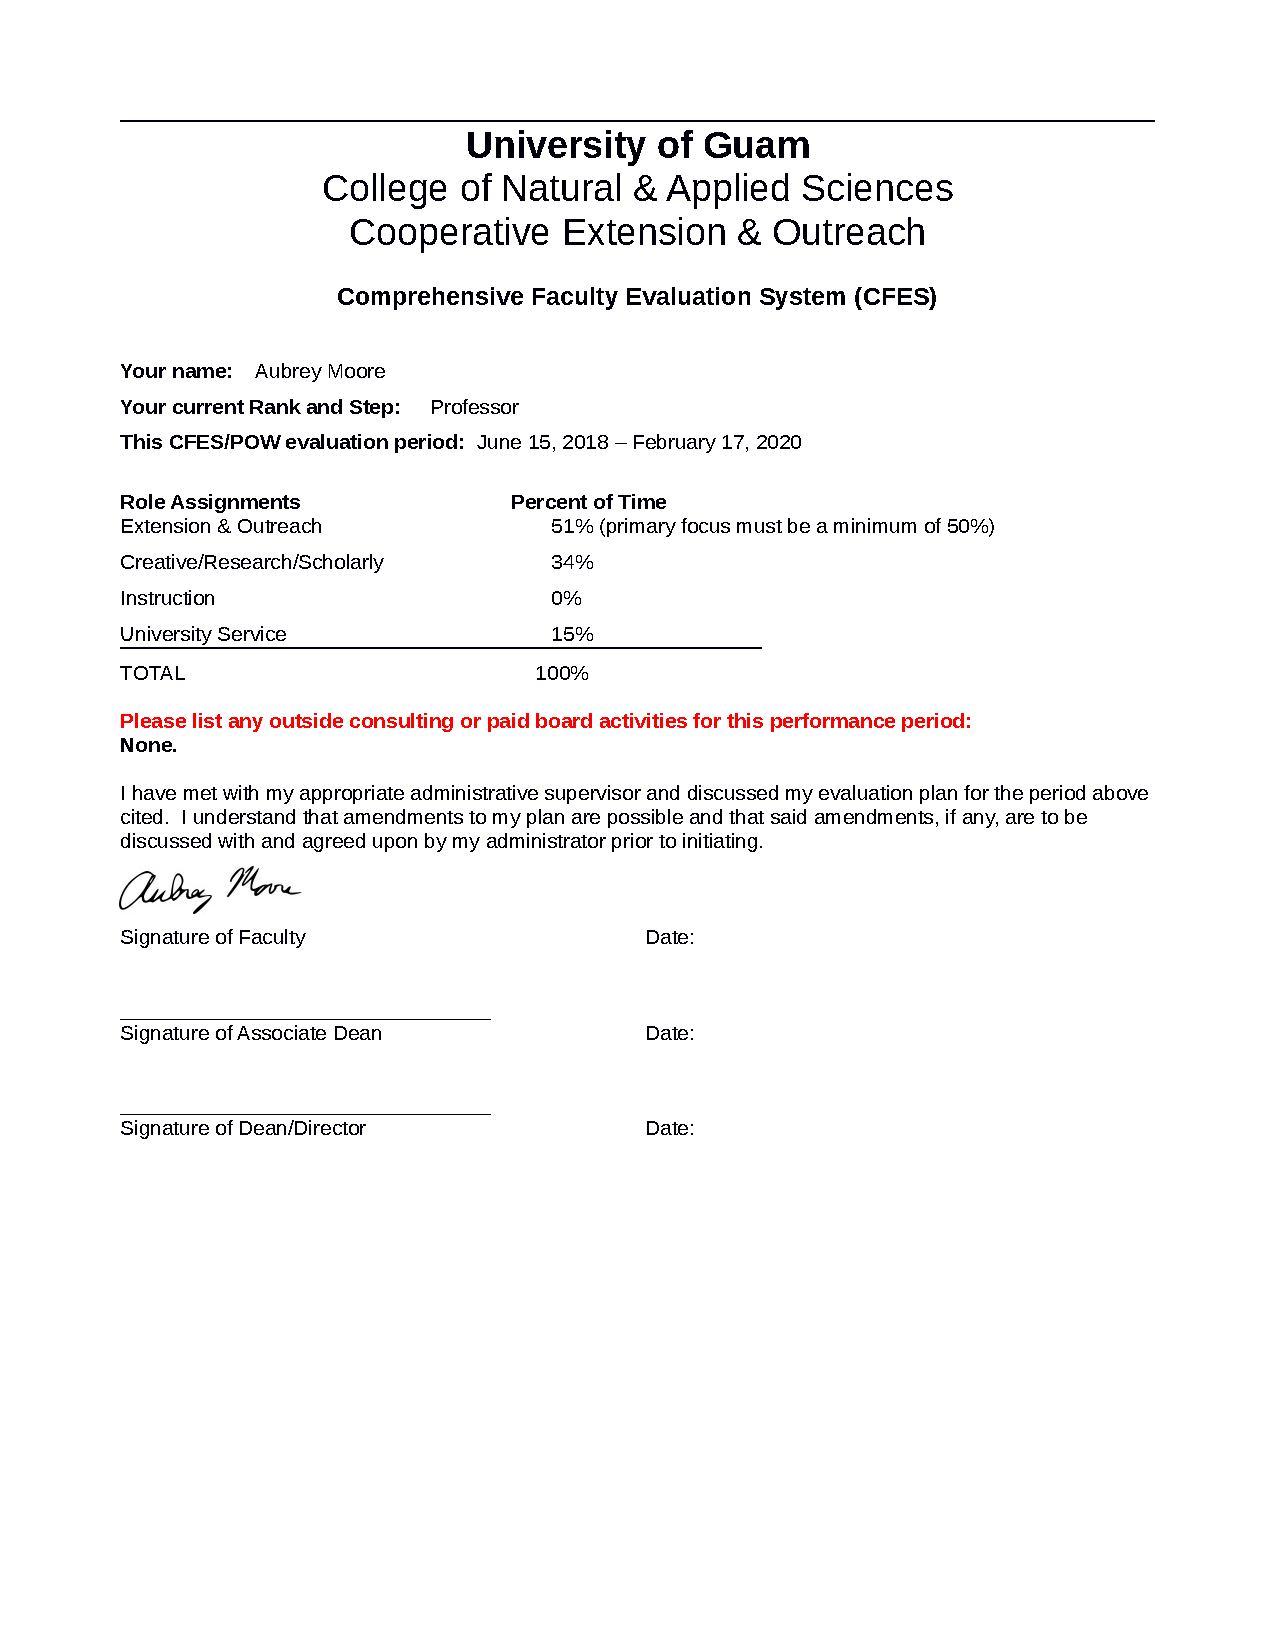
\includepdf[pages=1]{Reflective-form}

\setcounter{tocdepth}{2}
\tableofcontents{}

\clearpage

%\todo[inline]{add Guam beekeeper presentation}

\section{Preface}
	
I was hired by the University of Guam on October 1, 2003 under a limited-term,
split appointment (50\% extension and 50\% research). On June 26,
2008, I started a tenure-track appointment as extension entomologist
(100\% extension) with the academic rank of assistant professor. At
the end of the 2012 fall term I applied for tenure and promotion to associate professor and
received both in 2013. At the end of 2018 fall term I applied for promotion to
full professor and was promoted on July 11, 2019. 

I work within the Agriculture and Natural Resources Unit of the University
of Guam Cooperative Extension Service. I am a faculty member of the
Environmental Science Graduate Program and a member of the Western
Pacific Tropical Research Center. 

This report documents my activities during the period spanning June 15, 2020 to the present date.

My current faculty role allocation is as follows:
\begin{itemize}
	\item 51\% Extension and Community Activities 
	\item 34\% Creative/Scholarly Activity or Research 
	\item 15\% University and Community Service
\end{itemize}

\textbf{Note to Reader:}

This most recent version of this report is available as a PDF format which can be downloaded from \\
\url{https://github.com/aubreymoore/CFES2020-22/raw/main/CFES2020-22.pdf}. 

If you are reading the PDF version of this report on a device connected
to the internet, you will be able to follow hypertext links to documents
I have referenced.

\pagebreak

\section{Extension and Community Activities}

\subsection{Insect Diagnostic Services}
\begin{refsection}

\subsubsection{Description}	
As an extension entomologist, a major part of my job is providing
insect identification and pest control recommendations to a diverse
clientele including commercial growers, gardeners, householders, GovGuam
agencies, federal agencies, and UOG colleagues. Most client contacts
are initiated by a phone call or a visit by the client to the ANR
office. In many cases identification and pest control recommendations
require a site visit by me and/or extension associates to collect
samples and define the problem.

\subsubsection{Activities}

The number of extension calls requiring my assistance averaged approximately
one per day during the reporting period. Many of these are documented
as postings to iNaturalist \cite{moore_inat_since_2020-06-15}.

\subsubsection{Plans}

I plan to continue providing insect diagnostic services.

\subsubsection{References}

\printbibliography[heading=none]
\end{refsection}

\subsection{Detection and Documentation of Invasive Species}
\begin{refsection}

\subsubsection{Description}

Invasive insects are arriving on Guam at a very high rate (estimates
range as high as one new species per day). Very few of these are detected
and even fewer are identified because Guam suffers from \href{https://en.wikipedia.org/wiki/Taxonomic_impediment}{the taxonomic impediment}.
Even when reliable species determinations are made, new island records
are only rarely documented in the scientific press. Thus, impacts
of invasive insects on Guam and elsewhere in Micronesia are grossly
underestimated. One of my professional goals is to work towards solving
this problem by increasing the detection rate, getting specimens identified
by qualified taxonomists, and publishing new island records in the
scientific literature.

\subsubsection{Activities}

iNaturalist was used to document new records for insects detected in Guam and other Micronesian Islands \cite{inatSearch20220327}. 
Four new island records for insects in Micronesia were documented in iNaturalist posts during the reporting period \cite{inat108690775, inat103065598, inat57656025, inat48501627}.

\subsubsection{Plans}

I will continue to document new island records of insects detected in Micronesia.

The International Union for Conservation of Nature (IUCN-ISSG) is
building a Global Register of Introduced and Invasive Species. I have
volunteered to coordinate building a check list for species on Guam.

The Guam Invasive Species Council is required to maintain a list on
invasive species on Guam. I have volunteered to be ``registrar''
for this list.

\subsubsection{References}
\printbibliography[heading=none]
\end{refsection}

\subsection{University of Guam Insect Collection}
\begin{refsection}
	
\subsubsection{Description}

The UOG insect collection is a valuable reference collection for extension
entomology, teaching and research. I am a member of the board of directors
for the collection and I work with Dr. Ross Miller to curate and catalog
this collection.

In 2018 I ported the digital catalog for the UOG Insect Collection from a
CSIRO BioLink database to a more modern web-based Symbiota database
which is publicly available online \cite{moore_scan_2018}. I also established an internship to train entomology students how to curate an institutional insect collection and how to add specimen images to the digital catalog\cite{moore_internship_2018}. However, this work came to a halt because of space limitations. 

Facilities provided for the UOG insect collection are very poor. It is literally \textit{moth balled} in a small storage room which is too small for essential equipment such as microscopes and cameras. Curation and digitization necessitates removing specimens from the collection and transporting them outdoors to a lab where there is working space and equipment.

\subsubsection{Activities}

In May 2022, I arranged for EPSCOR funding to have a door installed between the UOG insect collection and the adjacent ANR lab. Access to bench space in the lab will partially solve the space limitation problem described in the preceding section. 


\subsubsection{Plans}

With the limited space problem partially solved, I intend to re-established the UOG insect collection internship to train entomology students how to curate an institutional insect collection.
The current focus will be on adding specimen images to the online database.

\subsubsection{References}
\printbibliography[heading=none]
\end{refsection}

\subsection{Mitigation of Damage to Guam's Ecosystems by Invasive Species}

Guam's ecosystems are rapidly being degraded by invasive species. These include:
\begin{itemize}
	\item \textbf{Brown treesnake} which has extirpated Guam's forest birds, causing loss of ecosystem services they provided, such as seed dispersal, insect control and pollination.
	\item \textbf{Cycad aulacaspis scale insect}, ACS, which has killed more than 90\% of Guam's endemic cycads, known locally as \textit{fadang}. Fadang went from being the most abundant plant in Guam's forests in 2002 to being listed as an endangered species in 2015.
	\item \textbf{Coconut rhinoceros beetle}, CRB, which is killing coconut palms and palma brava throughout the island. These two palm species where the second and third most abundant trees in Guam's forest in 2002. 
\end{itemize}

Clearly, an ecological disaster is happening on Guam, especially in forest ecosystems. As an extension entomologist, I am tasked with providing solutions to problems caused by insect pests. Unfortunately, there are no known methods for effectively controlling CAS and CRB on Guam. Therefor, I spend much of my time and effort performing applied research in an attempt to adequately control CAS and CRB so that restoration of Guam's forests can be attempted. 

\subsubsection{Activities}

Applied research is reported  in the Creative/Research/Scholarly: section \ref{sec:coconut-rhinoceros-beetle-(crb)-biocontrol} for CRB and section \ref{CASbiocontrol} for CAS.

\subsubsection{Plans}

I plan to continue providing control recommendations for invasive insect species when control methods are available.

I will continue with applied research on CAS and CRB in an effort to mitigate the major damage being done by these pests.

\subsection{National Plant Diagnostic Network (NPDN)}
\begin{refsection}

\subsubsection{Description}	

I serve as the UOG Coordinator for the National Plant Diagnostic Network (NPDN). UOG receives about \$15K per year from NPDN as a subrecipient of the Western Plant Diagnostic Network administered by UC Davis. Grant details are in  sections \ref{WPDN1}, \ref{WPDN2} and \ref{WPDN4YR}.

\subsubsection{Activities}

\begin{itemize}
	\item Participated in monthly conference calls.
	\item Prepared and submitted annual reports.
	\item Prepared a \href{https://github.com/aubreymoore/WPDN/blob/main/WPDN\%202021-2022\%20workplan\%20and\%20budget.pdf}{work plan and budget for FY2022}.
	\item Prepared a \href{https://github.com/aubreymoore/WPDN/raw/main/4year/WPDN\%20FY23-FY26\%20workplan\%20and\%20budget\%20for\%20UOG.pdf}{work plan and budget for FY2023-FY2026}.
	\item Attended the WPDN Annual Meeting in April 2022 via Zoom and made a presentation entitled \textit{The Invasive Species Problem on Guam} \cite{moore_invasive_2022}
\end{itemize}

\subsubsection{Plans}

I will continue to act as UOG coordinator for WPDN.

\subsubsection{References}
\printbibliography[heading=none]
\end{refsection}	



\subsection{Guam Invasive Species Advisory Committee (GISAC) and Guam Invasive Species Council (GISC)}
	
I am a founding member and regular participant in GISAC. President Underwood delegated me to represent UOG as a voting member of GISC and President Krise has reconfirmed my delegation.

\subsubsection{Activities}

I participated in GISAC and GISC meetings.

On Wednesday, November 17, 2021, I participated in a Guam Legislature Public hearing concerning biosecurity issues. I provided both written and oral testimony.

\subsubsection{Plans}

I plan to continue as an active member of GISAC and GISC.

I plan to participate in a review of the Guam Invasive Species Management Plan.

\subsection{Public Outreach: Internet}

Since the 1990s, I have built and maintained web sites to facilitate sharing information about insects in Micronesia. I created a wiki site to serve as an index to web resources I have developed (Available at  \url{https://guaminsects.net/aubwiki2020}). I will continue to use web sites to facilitate sharing information on Guam's insects.

\subsection{Public Outreach: Presentations}
\begin{refsection}
\nocite{moore_biological_2021, moore_how_2021,moore_presentation_2021}
\nocite{grasela_preliminary_2022}
\nocite{moore_invasive_2022}
\subsubsection{References}
\printbibliography[heading=none]
\end{refsection}

\subsection{Public Outreach: Miscelleaneous}
\begin{refsection}
\nocite{moore_what_2022}
\subsubsection{References}
\printbibliography[heading=none]
\end{refsection}

\subsection{Public Outreach: Public GitHub Repositories}

I attempt to provide access to as much of my work as possible using public GitHub repositories. GitHub is a free service for backing up and sharing documents on the web. Repositories which I have updated during the reporting period are listed in Table \ref{repolist}. Somewhere near the top of this list you will find a link to a repo called \textbf{CFES2020-22}. This repo contains the this document and all previous versions of the document.

I also use GitHub pages for serving static websites. A couple of good example sites are one which I created for my \href{https://aubreymoore.github.io/ALBI-345/}{ALBI345 General Entomology} course and one which is a \href{https://aubreymoore.github.io/crop-pest-list/}{List of Insects and Mites Attacking Crops in Micronesia}.

\begin{longtable}{ll}
\caption{List of GitHub repositories updated after 2020-06-15.}
\label{repolist}\\
\toprule
   updated &                                                                                                             repo \\
\midrule
\endfirsthead
\caption[]{List of GitHub repositories updated after 2020-06-15.} \\
\toprule
   updated &                                                                                                             repo \\
\midrule
\endhead
\midrule
\multicolumn{2}{r}{{Continued on next page}} \\
\midrule
\endfoot

\bottomrule
\endlastfoot
2022-08-05 &                   \href{https://github.com/aubreymoore/data-mining-insects-of-guam}{data-mining-insects-of-guam} \\
2022-08-04 &                                                   \href{https://github.com/aubreymoore/CFES2020-22}{CFES2020-22} \\
2022-07-30 &                                                                   \href{https://github.com/aubreymoore/POW}{POW} \\
2022-07-29 &                           \href{https://github.com/aubreymoore/2020-DOI-CRB-Biocontrol}{2020-DOI-CRB-Biocontrol} \\
2022-07-18 &                                           \href{https://github.com/aubreymoore/detection-range}{detection-range} \\
2022-07-01 &                   \href{https://github.com/aubreymoore/Guam-Forestry-Workshop-2022}{Guam-Forestry-Workshop-2022} \\
2022-06-30 &                                   \href{https://github.com/aubreymoore/sticky-trap-imaging}{sticky-trap-imaging} \\
2022-06-28 &                                             \href{https://github.com/aubreymoore/albi345-slides}{albi345-slides} \\
2022-06-23 &         \href{https://github.com/aubreymoore/Guam-Forestry-Workshop-Resources}{Guam-Forestry-Workshop-Resources} \\
2022-06-23 &                                                           \href{https://github.com/aubreymoore/crbdist}{crbdist} \\
2022-06-22 &                                                         \href{https://github.com/aubreymoore/CRB-FIDL}{CRB-FIDL} \\
2022-06-22 &                                                                   \href{https://github.com/aubreymoore/CAS}{CAS} \\
2022-06-16 &                                               \href{https://github.com/aubreymoore/gpepp_nursery}{gpepp_nursery} \\
2022-06-16 &                     \href{https://github.com/aubreymoore/sticky_traps_gpepp_nursery}{sticky_traps_gpepp_nursery} \\
2022-06-15 &                                         \href{https://github.com/aubreymoore/2022-06-09-drone}{2022-06-09-drone} \\
2022-05-30 &                                           \href{https://github.com/aubreymoore/good-vibrations}{good-vibrations} \\
2022-05-27 &                                                       \href{https://github.com/aubreymoore/treevibes}{treevibes} \\
2022-05-27 &                                                                 \href{https://github.com/aubreymoore/WPDN}{WPDN} \\
2022-05-25 &                                               \href{https://github.com/aubreymoore/guam-ias-bolo}{guam-ias-bolo} \\
2022-05-17 &                             \href{https://github.com/aubreymoore/CAS-biocontrol-seminar}{CAS-biocontrol-seminar} \\
2022-05-15 &                                                   \href{https://github.com/aubreymoore/inspireguam}{inspireguam} \\
2022-05-13 &                                                   \href{https://github.com/aubreymoore/inat_labels}{inat_labels} \\
2022-05-09 &                                                           \href{https://github.com/aubreymoore/SUMMA21}{SUMMA21} \\
2022-04-27 &                                                         \href{https://github.com/aubreymoore/WPDN2022}{WPDN2022} \\
2022-04-17 &             \href{https://github.com/aubreymoore/Tinian-sticky-traps-2022-02-26}{Tinian-sticky-traps-2022-02-26} \\
2022-04-07 &                                                     \href{https://github.com/aubreymoore/Tinian-CAS}{Tinian-CAS} \\
2022-03-24 &                                   \href{https://github.com/aubreymoore/Tinian-cycad-images}{Tinian-cycad-images} \\
2022-03-16 &                   \href{https://github.com/aubreymoore/Cave-micrographs-2022-03-16}{Cave-micrographs-2022-03-16} \\
2022-02-27 &                     \href{https://github.com/aubreymoore/sticky-trap-image-analysis}{sticky-trap-image-analysis} \\
2022-02-16 &                                             \href{https://github.com/aubreymoore/Harmonic-Radar}{Harmonic-Radar} \\
2021-12-17 &                                         \href{https://github.com/aubreymoore/McIntire-Stennis}{McIntire-Stennis} \\
2021-12-09 &                                           \href{https://github.com/aubreymoore/CRB-PPA19-Final}{CRB-PPA19-Final} \\
2021-12-07 &                         \href{https://github.com/aubreymoore/crb-diet-experiment-2021}{crb-diet-experiment-2021} \\
2021-12-07 &                   \href{https://github.com/aubreymoore/Guam-CRB-Damage-Map-2021-08}{Guam-CRB-Damage-Map-2021-08} \\
2021-12-06 &                                                         \href{https://github.com/aubreymoore/ALBI-345}{ALBI-345} \\
2021-12-04 &                                       \href{https://github.com/aubreymoore/FY19-PPA-Report-1}{FY19-PPA-Report-1} \\
2021-12-03 &                                                         \href{https://github.com/aubreymoore/bug-soup}{bug-soup} \\
2021-11-28 &   \href{https://github.com/aubreymoore/CRB-Action-Group-Webinar-2021-11-23}{CRB-Action-Group-Webinar-2021-11-23} \\
2021-11-27 &                                                   \href{https://github.com/aubreymoore/aubreymoore}{aubreymoore} \\
2021-11-26 &                                                             \href{https://github.com/aubreymoore/Guam05}{Guam05} \\
2021-11-21 &                                                         \href{https://github.com/aubreymoore/MCC-trap}{MCC-trap} \\
2021-10-24 &                                   \href{https://github.com/aubreymoore/github-repos-bibtex}{github-repos-bibtex} \\
2021-10-21 &                                           \href{https://github.com/aubreymoore/SWDC-2021-07-30}{SWDC-2021-07-30} \\
2021-10-19 &                                     \href{https://github.com/aubreymoore/aubrey_nikola_test}{aubrey_nikola_test} \\
2021-10-13 &                                                         \href{https://github.com/aubreymoore/pyzotero}{pyzotero} \\
2021-10-12 &                                                       \href{https://github.com/aubreymoore/GGI-Linux}{GGI-Linux} \\
2021-09-22 &                                           \href{https://github.com/aubreymoore/lecture-mimicry}{lecture-mimicry} \\
2021-09-20 &           \href{https://github.com/aubreymoore/lecture-insect-chemical-ecology}{lecture-insect-chemical-ecology} \\
2021-09-16 &                                                         \href{https://github.com/aubreymoore/open_pos}{open_pos} \\
2021-09-08 &                                                         \href{https://github.com/aubreymoore/groupImg}{groupImg} \\
2021-09-06 &                                                             \href{https://github.com/aubreymoore/mydemo}{mydemo} \\
2021-08-29 &                                             \href{https://github.com/aubreymoore/InsectWingbeat}{InsectWingbeat} \\
2021-08-21 &                                   \href{https://github.com/aubreymoore/Guam-CRB-damage-map}{Guam-CRB-damage-map} \\
2021-08-16 &                           \href{https://github.com/aubreymoore/InsectWingbeatWaveforms}{InsectWingbeatWaveforms} \\
2021-08-08 &                                                         \href{https://github.com/aubreymoore/wingbeat}{wingbeat} \\
2021-08-06 &                               \href{https://github.com/aubreymoore/USFS-Suggestions-2021}{USFS-Suggestions-2021} \\
2021-07-28 &                                       \href{https://github.com/aubreymoore/CRB-Import-Permit}{CRB-Import-Permit} \\
2021-07-22 &                                                 \href{https://github.com/aubreymoore/Pachodynerus}{Pachodynerus} \\
2021-07-13 &                                             \href{https://github.com/aubreymoore/cas-biocontrol}{cas-biocontrol} \\
2021-06-17 &                                                   \href{https://github.com/aubreymoore/cycad-scale}{cycad-scale} \\
2021-06-16 &                                                                 \href{https://github.com/aubreymoore/wiki}{wiki} \\
2021-06-14 &             \href{https://github.com/aubreymoore/2020-FS-CRB-biocontrol-project}{2020-FS-CRB-biocontrol-project} \\
2021-06-09 &                   \href{https://github.com/aubreymoore/top-10-most-costly-ias-mtcc}{top-10-most-costly-ias-mtcc} \\
2021-05-24 &             \href{https://github.com/aubreymoore/worlds-most-costly-ias-on-guam}{worlds-most-costly-ias-on-guam} \\
2021-05-24 &                   \href{https://github.com/aubreymoore/Guam-CRB-Damage-Map-2021-05}{Guam-CRB-Damage-Map-2021-05} \\
2021-05-18 &                                                         \href{https://github.com/aubreymoore/roadside}{roadside} \\
2021-04-24 &                   \href{https://github.com/aubreymoore/Guam-CRB-Damage-Map-2021-03}{Guam-CRB-Damage-Map-2021-03} \\
2021-04-14 &                           \href{https://github.com/aubreymoore/CRB-Project-Update-2021}{CRB-Project-Update-2021} \\
2021-03-29 &                                   \href{https://github.com/aubreymoore/crb-roadside-slides}{crb-roadside-slides} \\
2021-03-22 &                                       \href{https://github.com/aubreymoore/CRB-PPA19-Report3}{CRB-PPA19-Report3} \\
2021-03-22 &                             \href{https://github.com/aubreymoore/online-learning-course}{online-learning-course} \\
2021-03-18 &   \href{https://github.com/aubreymoore/CRB-Action-Group-Webinar-2021-03-17}{CRB-Action-Group-Webinar-2021-03-17} \\
2021-03-13 & \href{https://github.com/aubreymoore/University-of-Guam-Insect-Collection}{University-of-Guam-Insect-Collection} \\
2021-02-21 &                                                         \href{https://github.com/aubreymoore/CRB-CNMI}{CRB-CNMI} \\
2021-02-02 &                                             \href{https://github.com/aubreymoore/bts-mosquitoes}{bts-mosquitoes} \\
2021-01-27 &                   \href{https://github.com/aubreymoore/Guam-CRB-damage-map-2020-12}{Guam-CRB-damage-map-2020-12} \\
2021-01-13 &                     \href{https://github.com/aubreymoore/crb-roadside-impact-report}{crb-roadside-impact-report} \\
2021-01-12 &                                                   \href{https://github.com/aubreymoore/GGI-odonata}{GGI-odonata} \\
2020-12-19 &                                                         \href{https://github.com/aubreymoore/testhtml}{testhtml} \\
2020-12-10 &     \href{https://github.com/aubreymoore/CRBG-action-group-webinar-20201209}{CRBG-action-group-webinar-20201209} \\
2020-12-01 &                                             \href{https://github.com/aubreymoore/py4web-crb-app}{py4web-crb-app} \\
2020-11-24 &                 \href{https://github.com/aubreymoore/CRB-Damage-Survey-Validation}{CRB-Damage-Survey-Validation} \\
2020-11-23 &                                     \href{https://github.com/aubreymoore/new-crb-damage-map}{new-crb-damage-map} \\
2020-11-13 &                   \href{https://github.com/aubreymoore/Guam-CRB-damage-map-2020-10}{Guam-CRB-damage-map-2020-10} \\
2020-11-02 &                                       \href{https://github.com/aubreymoore/USAPI-Mosquito-ID}{USAPI-Mosquito-ID} \\
2020-10-15 &                                                             \href{https://github.com/aubreymoore/Guam01}{Guam01} \\
2020-09-17 &                                         \href{https://github.com/aubreymoore/roadside-article}{roadside-article} \\
2020-09-12 &                                   \href{https://github.com/aubreymoore/roadside-spatialite}{roadside-spatialite} \\
2020-09-04 &                                               \href{https://github.com/aubreymoore/PDF_to_Reveal}{PDF_to_Reveal} \\
2020-08-23 &                                 \href{https://github.com/aubreymoore/CRB-Damage-Detection}{CRB-Damage-Detection} \\
2020-07-10 &                                         \href{https://github.com/aubreymoore/Leo-Palace-Traps}{Leo-Palace-Traps} \\
2020-07-06 &                                                     \href{https://github.com/aubreymoore/qgiswebmap}{qgiswebmap} \\
2020-07-01 &                             \href{https://github.com/aubreymoore/Guam-Corona-Virus-Data}{Guam-Corona-Virus-Data} \\
2020-06-25 &                                 \href{https://github.com/aubreymoore/CRB-trap-improvement}{CRB-trap-improvement} \\
2020-06-21 &                                                                 \href{https://github.com/aubreymoore/temp}{temp} \\
\end{longtable}


\section{Creative/Scholarly Activities or Research}

\subsection{Peer Reviewed Publications (N=4)}
	\begin{refsection}
		\nocite{siderhurst_effects_2021, barrera_electron_2021, marshall_production_2021, cave_biological_2022}
		\printbibliography[heading=none]
	\end{refsection}

\subsection{Publication submitted for Peer Review (N=1)}
\begin{refsection}
	\nocite{moore_detecting_2022}
	\printbibliography[heading=none]
\end{refsection}

\subsection{Journal Articles in Preparation (n=5)}
\begin{refsection}
	
	\nocite{moore_first_nodate-1,moore_mariana_2013,moore_three_nodate-1,moore_change_nodate,moore_coconut_nodate-1}
	
	\printbibliography[heading=none]
\end{refsection}


\subsection{Coconut Rhinoceros Beetle (CRB) Biocontrol}\label{sec:coconut-rhinoceros-beetle-(crb)-biocontrol}
\begin{refsection}
	
\subsubsection{Description}

A newly discovered biotype of coconut rhinoceros beetle (CRB-G) is
rapidly killing coconuts and other palms on Guam and on other Pacific
islands. Following a failed eradication attempt on Guam, CRB-G proved
hard to control because it is resistant to \emph{Oryctes rhinoceros}
nudivirus (OrNV), which was previously used as the preferred biological
control agent for control of CRB outbreaks on Pacific Islands and
elsewhere. Prior to the discovery of CRB-G, all OrNV releases on
Pacific Islands resulted in immediate and sustained suppression of
CRB damage to low levels and prevented tree mortality.

Guam is currently experiencing an uncontrolled and unmonitored island-wide
CRB-G outbreak which was triggered by abundant CRB-G breeding sites
in the form of dead and dying vegetation left in the wake of Typhoon
Dolphin which occured in May 2015. of a recent typhoon. Most of these
breeding sites are inaccessable to sanitation efforts, being either
in the jungle or on military land (which covers one third of Guam).
A positive feedback cycle has begun whereby large numbers of adult
beetles are killing large numbers of palms which become breeding sites
which generate even higher numbers of adults. Severe damage to Guam\textquoteright s
palms prompted the Governor of Guam to declared a state of emergency
in July 2017.

The main objective of this project is to stop the uncontrolled outbreak
on Guam. Entomologists working on the CRB-G problem on several Pacific
islands agree that the most feasible tactic to halt tree mortality
and suppress damage to tolerable levels is establishment of biological
control using an isolate of OrNV which is highly effective as a biological
control agent for CRB-G. We are working with collaborators to identify
populations of CRB-G throughout the Asia-Pacific region. We will sample
these populations for biological control agent candidates which will
be evaluated in laboratory bioassays performed at UOG. Promising candidates
will be field released using autodissemmination as per a USDA-APHIS
import and release permit.

Concurrent with establishment of CRB-G biocontrol, success of the
project will be monitored in a quarterly, island-wide tree health
survey and incidence of OrNV infection will be monitored in a subsample
of all field collected CRB-G.

If the Guam CRB-G infestation cannot be controlled, it is expected
that most palms on the island will be killed and CRB-G will continue
to spread to other islands and beyond. If CRB-G invades smaller islands
and atolls where coconut is the tree of life, a human tragedy will
ensue. On larger islands, coconut and oil palm industries will be
severely impacted. Attempts to organize a well-funded, coordinated regional project in response to CRB-G have failed underway. However, UOG plays a major role in the \textit{ad hoc} CRB-G Action Group which was established to facilitate sharing scientific/technical information among people working on the CRB-G problem.

\subsubsection{Activities}

\paragraph{Funding and Project Management} This is my largest and most important project, requiring a lot of time and effort for project management including preparation of grant proposals and reports. During the reporting period, funding was provided by 4 grants totaling \$561,234: OIA-CRB [\ref{OIA-CRB}], APHIS-CRB [\ref{APHIS-CRB}], FS-CRB [\ref{FS-CRB}], and FS-CRB-HR [\ref{FS-CRB-HR}]. Details, including links to project proposals, work plans and progress reports are available in the grants section of this report.

\paragraph{Staffing}

Department of the Interior Office of Insular Affairs grant (OIA-CRB) supports Dr. James Grasela, an insect pathologist, and Christian Cayanan, a technician.

\paragraph{Establishment of a CRB Rearing Facility and Rearing Protocol}

Development of biocontrol for CRB-G will require laboratory bioassays using standardized, healthy lab-reared beetles of equivalent age. Previously, we used beetles collected from pheromone traps for this purpose. However, mortality in experimental control groups was highly variable, yeilding irreproducible results. 

During the reporting period:
\begin{itemize}
	\item We built and equipped a CRB rearing facility in a 40 foot shipping container.  
	\item We developed and tested a natural larval diet by grinding dead standing coconut stems containing CRB breeding sites.
\end{itemize}

\paragraph{Establishment of an Island-wide CRB Damage Monitoring System}

We developed an island-wide roadside monitoring system to track spatial and temporal changes in CRB damage levels. Data are collected using a smart phone attached to a project vehicle. The phone continually records georeferenced roadside images as the vehicle is driven along all major results in both directions. Data are automatically analysed by an image analysis system which detects coconut palms in the images, calculates a damage index for each palm, and outputs results on a map of Guam. A nontechnical overview of this system was published in the 2020 WPTRC Impact Report \parencite{moore_using_2020-1}.

To date, we have completed five surveys and data for a sixth have been recorded. Interactive damage maps are available on the web: 
\begin{itemize}
	\item October 2020  \parencite{moore_crb_2020-1}
	\item December 2020 \parencite{moore_crb_2020}
	\item March 2021 \parencite{moore_crb_2021} 
	\item May 2021 \parencite{moore_crb_2021-1}
	\item August 2021 \parencite{moore_crb_2021-2}	
\end{itemize}


%\paragraph{Current focus} is on finding an isolate of \textit{Oryctes} rhinoceros nudivirus which can be used as a biological control agent for CRB-G. Laboratory bioassays have identified one OrNV isolate which is potential candidate and further tests are under way.
%
%I have developed an online database to facilitate record keeping and report generation for CRB rearing and bioassays \cite{moore_coconut_2019-1}. 
%
%Dr. Grasela has worked in coordination with Dr. Hui Jiang to build DNA diagnostics capacity. We can now test for OrNV in individual beetles.

\paragraph{International collaboration} will be essential for finding a way to halt massive ecological and economic damage to Pacific islands invaded by CRB-G. A CRB-G Action Group was formed was formed to facilitate collaboration and cooperation. prior to COVID, this group met annually at international scientific meetings. During COVID, I helped to keep the group together by hosting Zoom webinars with assistance from the UOG Office of Information Technology. I created web pages to facilitate access recordings of these webinars: 
\begin{itemize}
	\item March 17, 2021 \cite{moore_video_2021-1}
	\item December 9, 2020 \cite{moore_video_2020}
	\item November 23, 2021 \cite{moore_video_2021}	
\end{itemize}

\paragraph{Outreach} In an effort to facilitate technical and scientific information among people working on CRB, we have developed and maintain several online resources including a wiki \parencite{moore_crb-g_2019}, a Facebook site \parencite{moore_facebook_2019}, an online interactive map of CRB invasion history \parencite{moore_online_2019} and a CRB reference library \parencite{moore_online_2021}, and an online email discussion site \parencite{moore_online_2021-1}.

\paragraph{Harmonic radar}
%\begin{refsection}
I am investigating the feasibility of using harmonic radar using funding from a US Forest Service grant [\ref{FS-CRB-HR}]. Details of this applied research are available as a preprint journal article \cite{moore_detecting_2022}. This work is being done in collaboration with Dr. Matt Siderhurst, a chemical ecologist at Eastern Mennonite University, Virginia. I am also collaborating with Dr. Glenn Dulla, Guam Department of Agriculture on the feasibility of using a harmonic radar unit attached to a drone. 			
%\printbibliography[heading=none]
%\end{refsection}
		
\paragraph{CRB-G tissue culture}
%\begin{refsection}
The project's insect pathologist has established a tissue culture of CRB-G cells \cite{grasela_preliminary_2022}.
This cell line may be useful for in vitro production of \textit{Oryctes rhinoceros} nudivirus which is currently propagated in a cell line from a different scarab beetle.
%\printbibliography[heading=none]
%\end{refsection}

\subsubsection{Plans}

Plans for this project are contingent on applied research results, availability of funding and availability of resources.

\paragraph{Funding} 

Three of the four grants supporting this project, terminate within calendar year 2022. The remaining grant, DOI-OIA [\ref{OIA-CRB}], terminates on September 30, 2023. I do not have plans to apply for additional grant funding for this project.

\paragraph{Staffing}

The project's insect pathologist, Dr. Jim Grasela, is resigning on June 24, 2022. Recruitment of additional scientific/technical help will be required.

\paragraph{CRB-G biocontrol} 

We will continue performing bioassays until a potential OrNV biocontrol candidate is found. Once we have one, we will begin propagation \textit{in vivo} and field releases via autodissemination. I already have a USDA-APHIS permit for field release of OrNV.

The current priority is to perform a critical laboratory bioassay to test for significant reduction in fecundity (egg laying) caused by OrNV isolate V23B. This isolate caused significant mortality in bioassays performed in our lab and also in the Solomon Islands. However, according to some of the literature, the main mode of action causing population reduction by OrNV is not mortality but reduction in fecundity. Given the long lifespan of CRB, this experiment will require at least a year (includes lab rearing of test insects).

\paragraph{Island-wide CRB Damage Surveys} We will continue island-wide CRB damage surveys.

\paragraph{Harmonic radar} The field trial detailed in the work plan for my grant [\ref{FS-CRB-HR}] will be done during the first two weeks of July 2022. 

\paragraph{CRB-G tissue culture} We will attempt to have another lab adopt the CRB-G cell line culture prior to Dr. Grasela's departure from UOG.

\subsubsection{References}
\printbibliography[heading=none]

\end{refsection}


\subsection{Guam Biodiversity Inventory}
\begin{refsection}
	
	\subsubsection{Description}
	
	I consider this to be my second most important project.
	
	A biodiversity inventory is essentially a database containing a comprehensive
	check list of all taxa known occur within a defined area.
	
	A terrestrial biodiversity inventory for Guam is needed to document
	rapid changes to Guam's ecosystems, to provide free
	and open access to information on Guam's flora and
	fauna, and to share Guam biodiversity information with the global
	scientific community, policy makers and the public.
	
	The Guam Biodiversity Inventory will facilitate automatic generation
	and updates to lists such as: a list of all invasive species on Guam
	with year first recorded, a list of new species described from specimens
	collected on Guam, a list of observations for Guam's
	endangered species, a list of Guam's native plants
	with associated herbivores and pathogens, and a list of crops grown
	on Guam and pests and pathogens which attack them.
	
	\subsubsection{Activities}
	
	\paragraph{Funding} This project is supported by my McIntire-Stennis grant \ref{BIODIVERSITY} which terminates on 2022-09-30.
	
	\paragraph{Staffing} I offered an internship to work on this project to Annette Kang, a graduate student from Guam currently working on a PhD in Entomology at Cornell University. Progress on this project was impeded because of a nine month delay in processing my interns stipend payment.  	
	
	\paragraph{Data mining} During the reporting period, the focus within this project was to extract data from legacy entomological literature for Guam, namely \textit{Insects of Guam} I and II. This work was facilitated using a sophisticated workflow developed by \href{https://en.wikipedia.org/wiki/Plazi}{Plazi}, a Swiss-based international non-profit association supporting and promoting the development of persistent and openly accessible digital biodiversity information. The Plazi office in Brazil kindly supported this project by provided online training sessions for myself and Annette. Data extracted from the literature are automatically published on the Global Biodiversity Information Facility as datasets and occurrence records. I wrote an \href{https://aubreymoore.github.io/data-mining-insects-of-guam/MatCit-Validator/status_report.html}{online dashboard to track our data-mining progress}. More details are available in my 2021 annual report for this project \cite{moore_guam_2021}
	
	\subsubsection{Plans}
	
	I am working to complete this project before the grant expires on 2022-09-30 and to complete a final report due 2022-12-31.
	
	\subsubsection{References}
	\printbibliography[heading=none]
\end{refsection}

%\subsection{Guam Forest Insect Survey}
%\begin{refsection}
%	
%	\subsubsection{Description}
%	
%	The objective of this project is to compile a comprehensive check
%	list of insects impacting Guam's forests. While it is notable that
%	Guam's two most numerous forest trees, namely fadang, \emph{Cycas
%		micronesica}, and coconut palm, \emph{Cocos nucifera}, are under simultaneous
%	attack by invasive insects, there are many other forest plants under
%	attack from invasive insects. This project is funded by McIntire-Stennis.
%	
%	\subsubsection{Activities}
%	
%	This grant was completed in 2018. See final report \cite{moore_aubreymoore/mcintire-stennis_2018}.
%		
%	\subsubsection{Plans}
%	
%	None. This grant project has been completed.
%	
%	\subsubsection{References}
%	\printbibliography[heading=none]
%\end{refsection}


\subsection{Cycad Aulacaspis Scale (CAS) Biocontrol}
\label{CASbiocontrol}
\begin{refsection}

\subsubsection{Description}

A US Forest Service survey published in 2002 reported that the most
abundant tree in Guam's forests (DBH > 5 inches) was Guam's endemic
cycad, \emph{Cycas micronesica}. In 2003, an invasive scale insect,
\emph{Aulacaspis yasumatsui}, was detected on ornamental cycads but
it soon infested wild cycads and started killing them. Within a decade,
90\% of Guam\textquoteright s endemic cycads have been killed by the
scale and other invasive species. \emph{Cycas micronesica} was placed
on the US National Endangered Species List in 2015.

Mature plants are protected by a lady beetle I introduced, but no
natural reproduction of the cycads is occurring because seeds and seedlings are
still being killed by the scale insect. A likely solution to this
problem is establishment of a small biocontrol agent, such as a miniature
parasitic wasp, which will control scale insects infesting seeds and
seedlings.

\subsubsection{Activities}

I collaborated with Dr. Jim McConnell on insect pests impacting cycads on Tinian and Guam. I set up a pest monitoring of cycads in conservation plots on Tinian using leaf samples \cite{moore_monitoring_2022} and yellow sticky traps \cite{moore_monitoring_2022-1}.

In March 2022, I hosted a visit from Dr. Ron Cave from the University of Florida. Ron is an expert on CAS biocontrol and I have been trying to get him out here on a consulting trip for several years. Some discussions with USFWS earlier this year led to them funding the trip.

During his trip, Ron and I hosted a Zoom seminar on CAS biocontrol. I put recordings of the presentations and discussion online \cite{cave_biological_2022-1}. After the trip, Dr. Cave provided \href{https://github.com/aubreymoore/CAS-biocontrol-seminar/raw/main/Cave-CAS-report-2022.pdf}{comprehensive consulting report complete with recommendations}. 

In addition, I coauthored a book chapter on CAS biocontrol with Ron Cave and Mark Wright, University of Hawaii \cite{cave_biological_2022}.

\subsubsection{Plans}

I will work to help find funding to implement Dr. Cave's recommendations. My work on CAS biocontrol is currently unfunded.

\subsubsection{References}
\printbibliography[heading=none]

\end{refsection}


\subsection{Eight Spot Butterfly (ESB) Conservation}
\begin{refsection}

\subsubsection{Description}

The Guam Department of Agriculture Division of Aquatic and Wildlife
Resources (GDOA-DAWR) requested assistance with conservation of the
rare Mariana eight-spot butterfly, \emph{Hypolimnas octocula marianensis}. I prepared a grant proposal and a permit application to do this work under a cooperative agreement with the GDOA-DAWR.

The objective of this project is to investigate the feasibility of captive rearing.

\subsubsection{Activities}

I have partnered with Dr. Curt (George) Fiedler, Biology Department, and the Center for Island Sustainability to collaborate on this project.

A large field cage (20x20X10 feet) has been built in the UOG Center for Island Sustainability compound in Dean's Circle and a shade house has been stocked with host plants. 

On 2020-05-25, I organized a Zoom conference call with the US Fish and Wildlife Service to discuss conditions of a new permit which will allow UOG and the Guam Department of Agriculture - Division of Aquatic and Wildlife Resources to work on captive breeding of the Mariana eight-spot butterfly.

\subsubsection{Plans}

Breeding experiments will commence within the next 2 months.

\end{refsection}


%\subsection{Development of a Camera Trap for Insects}
%\begin{refsection}
%\subsubsection{Description}
%
%The objective of this project is to build a camera trap which uses motion detection to automatically capture short videos of active insects.
%
%The initial target application is a surveillance system for insects visiting flowers.
%
%\subsubsection{Activities}
%
%Initial attempts at hardware and software development are available on an Open Science Framework site \cite{moore_development_2019} and in a GitHub repository \cite{moore_github_2019-2}.
%
%\subsubsection{Plans}
%
%For the first target application of this technology, I am partnering with Dr. Jim McConnel and staff of the Guam Plant Extinction Prevention Project to discover insect pollinators of an endangered endemic plant.
%
%I plan to test the camera trap for monitoring bee hive activity, including detecting arrival of hornets (\textit{Vespa tropica}).
%
%USDA-APHIS herpetologist, Dr. Shane Sears, has asked me to collaborate with him on developing digital image analysis of brown tree snake videos.
%
%\subsubsection{References}
%\printbibliography[heading=none]
%\end{refsection}

\pagebreak
\section{University and Community Service}

\subsection{Undergraduate Instruction}
\begin{refsection}
	
\subsubsection{Description}

In addition to fulfilling my primary role as an extension entomologist, I am required to teach undergraduate courses.

\subsubsection{Activities}


\paragraph{AL/BI 345 General Entomology}
During Fall term 2021, I taught the lecture and laboratory sections of AL/BI 345 General Entomology.

I prepared a syllabus for this course \cite{moore_syllabus_2021}. I also built and maintained a web site \cite{moore_web_2021} and populated this with lecture notes and other resources.  My scores in the student evaluations for all 4 course sections were consistently higher than both university and college averages \cite{moore_instructor_2021}.

\paragraph{Special Project for Laura Caser, Biology}
I am currently supervising biology student Laura Caser on a special project. She is recording and analyzing coconut rhinoceros beetle feeding sounds using a new bioacoustics sensor called TreeVibes.

\paragraph{Summer Workshop on Mathematical Modelling}

During June and July 2021, I assisted in teaching undergraduates and high school students in a summer workshop on mathematical modeling of ecological systems. The program was coordinated by Dr. Hyunju Oh, UOG Mathematics, and funded by three of her grants: GECCO Summer Math Research Experience (SMRE), National Research Experience for Undergraduates Program (NREUP), and Young Scholars Research Experience in Mathematics (YSREM). I provided lectures and assistance to teams of students modelling \textit{Invasion of the Coconut Rhinoceros Beetle (CRB) on Guam}.

My lectures and resource materials were made available in GitHub web page at \url{https://aubreymoore.github.io/SUMMA21/}.

\subsubsection{Plans}

None

\subsubsection{References}
\printbibliography[heading=none]
\end{refsection}

\subsection{Graduate Instruction}

I am a member of the Graduate Faculty of the Environmental Sciences Program. During the reporting period, I frequently presented guest lectures for EV courses. I also served as a member of Chris Rosario's masters committee and I have agreed to serve on the committee of a new maters student, Caylin McCormick.

I serve on the masters committee of Matt Putnam, a biology student working on captive breeding of the Marianas eight-spot butterfly. 

\subsection{Faculty Committees}

\subsubsection{Faculty Building Facilities Committee for the ALS}

This committee was formed by the Agriculture and Life Sciences Division
to consult with the Dean on facilities problems within the Agriculture
and Life Sciences Building. I was re-elected as chair of this committee, joined by Dr. Jim McConnell.

\raggedright\vspace{2mm}\textbf{Activity}
	
The committee's biggest accomplishment during the reporting period was installation of Prometheus smart screens in ALS 124 and ALS 127.

\subsubsection{Search Committee: Restoration Ecologist}

I currently serve on a search committee for the new Restoration Ecologist position in the Biology department with Dr. Dan Lidstrom (Chair) and Dr. Frank Camacho.

\subsubsection{Search Committee: Research Associates for RCUOG Brown Treesnake Grants}

I was a member of several search committees for BTS technicians. I was joined by Dr. Shane Siers(PI and Chair) and Dr. Dan Lindstrom.
\begin{itemize}
	\item Feb 2021: Research Associate I
    \item Jun 2021: 2x Research Assistant I
    \item Jul 2021: Research Associate I
	\item Mar 2022: 2x Research Associate I
\end{itemize}


\newpage
\section{Grants which were active during the reporting period (n=8)}

Note: Five grants terminate before the end of 2022.

\begin{table}[h!]
	\centering
	\caption{List of grants active during the reporting period (2020-06-15 through 2022-06-15).}
	\label{grantlist}
	\begin{tabular}{lp{3in}>{\raggedleft\arraybackslash}l}
		\toprule
		code &                                                                                                    title &  funding \\
		\midrule
		OIA-CRB (\ref{OIA-CRB}) & Establishment of Self-sustaining Biological Control of Coconut Rhinoceros Beetle Biotype G in Micronesia & \$239,994 \\
		\midrule
		APHIS-CRB(\ref{APHIS-CRB}) &                                        Biological Control of Coconut Rhinoceros Beetle Biotype G on Guam & \$200,000 \\
		\midrule		
		FS-CRB (\ref{FS-CRB})& Establishment of Self-sustaining Biological Control of Coconut Rhinoceros Beetle Biotype G in Micronesia &  \$98,240 \\
		\midrule
		BIODIVERSITY (\ref{BIODIVERSITY}) &                                                                       Guam Forest Biodiversity Inventory &  \$80,000 \\
		\midrule		
		WPDN1 (\ref{WPDN1}) &                                                                         Western Plant Diagnostic Network &  \$63,366 \\
		\midrule
		8SPOT (\ref{8SPOT}) &                                                                 Captive Breeding of Eight-spot Butterfly &  \$23,212 \\
		\midrule
		FS-CRB-HR (\ref{FS-CRB-HR})&                         Improving Coconut Rhinoceros Beetle Breeding Site Detection Using Harmonic Radar &  \$23,000 \\
		\midrule
		WPDN2 (\ref{WPDN2}) &                                                                  Western Plant Diagnostic Network FY2022 &  \$15,000 \\
		\bottomrule
	\end{tabular}
\end{table}

\begin{figure}[h!]
\label{gannt}
\begin{ganttchart}[time slot format=isodate, expand chart=\textwidth]{2020-01-01}{2023-12-31}
%	\gantttitle{2011}{12} \\
	\gantttitlecalendar{year} \\
	\ganttgroup{reporting period}{2020-06-15}{2022-06-15} \\
	\ganttbar{APHIS}{2020-01-01}{2021-08-07} \\
	\ganttbar{DOI-OIA}{2020-06-15}{2023-09-30} \\
	\ganttbar{McStennis}{2020-05-14}{2022-09-30}\\
	\ganttbar{8spot}{2020-01-01}{2022-09-30}\\
	\ganttbar{WPDN1}{2020-01-01}{2021-07-31}\\
	\ganttbar{WPDN2}{2021-09-01}{2022-08-31}\\
	\ganttbar{FS-HR}{2020-06-17}{2022-12-31}\\
	\ganttbar{FS-CRB}{2020-06-17}{2022-12-31}		
	\ganttvrule{}{2020-06-15}
	\ganttvrule{}{2021-06-15}
	\ganttvrule{}{2022-06-15}
\end{ganttchart}
\caption{Performance periods for grants which were active during the reporting period (2020-06-15 through 2022-06-15).}
\end{figure}





\clearpage
\subsection{APHIS-CRB Biological Control of Coconut Rhinoceros Beetle Biotype-G \$200K}
\label{APHIS-CRB}

\subsubsection{Key data}
\begin{itemize}
	\setlength\itemsep{0em}
	\item \textbf{Code:} APHIS-CRB
	\item \textbf{Long title:} Biological Control of Coconut Rhinoceros Beetle Biotype G on Guam	
	\item \textbf{Start date:} 2019-08-08	
	\item \textbf{End date:} \textcolor{red}{2021-08-07}	
	\item \textbf{Total budget:} \$200,000	
	\item \textbf{Federal ID:} AP19PPQS\&T00C168
	\item \textbf{UOG ID:} USDA Biocontrol 2019
	\item \textbf{UOG Account:} 30-2F-311117
	\item \href{https://github.com/aubreymoore/FY19-PPA-Report-1}{GitHub repository}
\end{itemize}

\subsubsection{Documents}
\begin{itemize}
	\setlength\itemsep{0em}	
	\item \href{https://github.com/aubreymoore/Miscellaneous-Docs-for-CFES2018/raw/master/MooreFB19.pdf}{Proposal}		
	\item \href{https://github.com/aubreymoore/FY2018-Farm-Bill-Suggestion/blob/master/from\%20EFG/Award\%20Document.pdf}{Award letter}			
	\item \href{https://github.com/aubreymoore/FY2018-Farm-Bill-Suggestion/raw/master/extension-request/MooreFB19WorkPlan-ammended.pdf}{Ammended work plan}		
	\item \href{https://github.com/aubreymoore/FY19-PPA-Report-1/raw/master/PPA19-report-1.pdf}{Report 1}	
	\item \href{https://github.com/aubreymoore/FY19-PPA-Report-1/raw/master/PPA19-report2.pdf}{Report 2}		
	\item \href{https://github.com/aubreymoore/CRB-PPA19-Report3/blob/main/PPA19-report3.pdf}{Report 3}		
	\item \href{}{Final Report}
\end{itemize}




\clearpage
\subsection{OIA-CRB Biological Control of Coconut Rhinoceros Beetle Biotype-G in Micronesia \$177K}
\label{OIA-CRB}

\subsubsection{Key data}
\begin{itemize}
	\setlength\itemsep{0em}	
	\item \textbf{Code:} OIA-CRB
	\item \textbf{Title:} Establishment of Self-sustaining Biological Control of Coconut Rhinoceros Beetle Biotype G in Micronesia
	\item \textbf{Start date:} 2020-05-14
	\item \textbf{End date:} 2023-09-30
	\item \textbf{Total budget:} \$239,994
	\item \textbf{Federal ID:} D20AP00060
	\item \textbf{UOG ID:} DOI Biocontrol CRB
	\item \textbf{UOG Account:} 30-2F-311150
	\item \href{https://github.com/aubreymoore/2020-DOI-CRB-Biocontrol}{GitHub repository}
\end{itemize}

\subsubsection{Documents}
\begin{itemize}
	\setlength\itemsep{0em}	
	\item \href{https://github.com/aubreymoore/2020-DOI-CRB-Biocontrol/blob/master/doi_proposal.pdf}{Proposal}
	\item \href{https://github.com/aubreymoore/2020-DOI-CRB-Biocontrol/blob/master/D20AP00060-Grant\%20Award\%20Document.pdf}{Award letter}
	\item \href{https://github.com/aubreymoore/2020-DOI-CRB-Biocontrol/raw/master/Reporting\%20requirements\%20\%20D17AP00107.pdf}{Reporting requirements}
	\item \href{https://github.com/aubreymoore/2020-DOI-CRB-Biocontrol/raw/master/doi_report1.pdf}{Report 1}
\end{itemize}

\newpage
\subsection{BIODIVERSITY Guam Forest Biodiversity Inventory \$80K}
\label{BIODIVERSITY}
\subsubsection{Key data}
\begin{itemize}
	\setlength\itemsep{0em}
	\item \textbf{Code:} BIODIVERSITY
	\item \textbf{Title:} Guam Forest Biodiversity Inventory
	\item \textbf{Funding source:} McIntire-Stennis (administered by CNAS)
	\item \textbf{Reporting system:} \href{https://portal.nifa.usda.gov/portal/front/login}{REEport}
	\item \textbf{Start date:} 2018-10-15
	\item \textbf{End date:} 2022-09-30
	\item \textbf{Total budget:} \$16,000 per year for each of 4 years
	\item \textbf{Federal ID:} GUA0930
	\item \textbf{UOG ID:}
	\item \textbf{UOG Account:}
	\item \href{https://github.com/aubreymoore/McIntire-Stennis}{GitHub repository}
\end{itemize}

\subsubsection{Documents}
\begin{itemize}
	\setlength\itemsep{0em}	
	\item \href{https://github.com/aubreymoore/McIntire-Stennis/raw/master/MS_Project_Proposal_2018/ms_proposal_2018.pdf}{2018-06-21 Proposal}
	\item \href{https://github.com/aubreymoore/McIntire-Stennis/raw/master/project_initiation.pdf}{2018-10-08 Project initiation}
	\item \href{https://github.com/aubreymoore/McIntire-Stennis/raw/master/2019-report.pdf}{2020-01-02 2019 Annual report}
	\item \href{https://github.com/aubreymoore/McIntire-Stennis/raw/master/2020\%20Annual\%20Report/2020\%20McS\%20Annual\%20Report.pdf}{2020-12-28 2020 Annual report}
	\item \href{https://github.com/aubreymoore/McIntire-Stennis/raw/master/2021\%20Annual\%20Report/submitted_for_review.pdf}{2021-12-18 2021 Annual report}
	\item Final report due 2022-12-31.
\end{itemize}





\newpage
\subsection{8SPOT Eight Spot Butterfly Conservation \$20K}
\label{8SPOT}
\subsubsection{Key data}
\begin{itemize}
	\setlength\itemsep{0em}
	\item \textbf{Code:} 8SPOT
	\item \textbf{Title:} Captive Breeding of Eight-spot Butterfly
	\item \textbf{Start date:} 2013-10-01
	\item \textbf{End date:} 2022-09-30
	\item \textbf{Total budget:} \$23,212
	\item \textbf{Funding Agency:} DOI-FWS (via GDOA-DAWR)
	\item \textbf{Federal ID (FAIN):} F13AF01300
	\item \textbf{UOG ID:}
	\item \textbf{UOG Account:} 30-1F-315058-R
	\item \href{https://github.com/aubreymoore/Hypolimnas-octocula-conservation}{GitHub repository}
\end{itemize}

\subsubsection{Documents}
\begin{itemize}
	\setlength\itemsep{0em}	
	\item \href{https://github.com/aubreymoore/Hypollimnas-octocula-conservation/blob/master/8spot-award-notice.pdf}{Award letter (includes scope of work and budget)}
	\item \href{https://github.com/aubreymoore/Hypollimnas-octocula-conservation/blob/master/8spot-award-notice-updated.pdf}{Updated Award Letter}
\end{itemize}





\newpage
\subsection{WPDN1 Western Plant Diagnostic Network 2016 \$63K}
\label{WPDN1}

\subsubsection{Key data}
\begin{itemize}
	\setlength\itemsep{0em}	
	\item \textbf{Code:} WPDN1
	\item \textbf{Long title:} Western Plant Diagnostic Network
	\item \textbf{Start date:} 2016-09-01
	\item \textbf{End date:} \textcolor{red}{2021-07-31}
	\item \textbf{Total budget:} \$63,366
	\item \textbf{Federal ID(FAIN):} 20163762025851
	\item \textbf{UOG ID:}
	\item \textbf{UOG Account:} 2F-243432R5
	\item \href{https://github.com/aubreymoore/WPDN}{GitHub repository}
\end{itemize}

\subsubsection{Documents}
\begin{itemize}
	\setlength\itemsep{0em}	
	\item \href{https://github.com/aubreymoore/WPDN/raw/main/WPDN\%20-award-2020.pdf}{Proposal and Award Letter}
\end{itemize}





\newpage
\subsection{WPDN2 Western Plant Diagnostic Network FY2022 \$15K}
\label{WPDN2}

\subsubsection{Key data}
\begin{itemize}
	\setlength\itemsep{0em}	
	\item \textbf{Code:} WPDN2
	\item \textbf{Title:} Western Plant Diagnostic Network FY2022
	\item \textbf{Start date:} 2021-09-01
	\item \textbf{End date:} 2022-08-31
	\item \textbf{Total budget:} \$15,000
	\item \textbf{UOG ID:} WPTRC-UCDAVIS/USDA WPLANTDI
	\item \textbf{UOG Account:} 61-1F-243432
	\item \href{https://github.com/aubreymoore/WPDN}{GitHub repository}
\end{itemize}

\subsubsection{Documents}
\begin{itemize}
	\setlength\itemsep{0em}	
	\item \href{https://github.com/aubreymoore/WPDN/blob/main/WPDN\%202021-2022\%20workplan\%20and\%20budget.pdf}{Work plan and budget}
	\item \href{https://github.com/aubreymoore/WPDN/raw/main/FY2022/WPDN-FY2022-Award-Letter.pdf}{Award letter}
	\item \href{https://github.com/aubreymoore/WPDN/raw/main/FY2022/UOG-account-setup.pdf}{UOG account setup}
\end{itemize}





\newpage
\subsection{FS-CRB-HR Harmonic Radar \$23K}
\label{FS-CRB-HR}

\subsubsection{Key data}
\begin{itemize}
	\setlength\itemsep{0em}
	\item \textbf{Code:} FS-CRB-HR
	\item \textbf{Long title:} Improving Coconut Rhinoceros Beetle Breeding Site Detection Using Harmonic Radar
	\item \textbf{Start date:} 2020-06-17
	\item \textbf{End date:} 2022-12-31
	\item \textbf{Total budget:} \$23,000
	\item \textbf{Federal ID:} 20-DG-11052021-227
	\item \textbf{UOG ID:} CNAS-USDA-CRB Harmonic Radar
	\item \textbf{UG Account:} 30-2F-311144-R
	\item \href{https://github.com/aubreymoore/Harmonic-Radar}{GitHub repository}
\end{itemize}

\subsubsection{Documents}
\begin{itemize}
	\setlength\itemsep{0em}		
	\item \href{https://github.com/aubreymoore/Harmonic-Radar/blob/master/USFS-harmonic-radar-proposal.pdf}{Proposal}
	\item \href{https://github.com/aubreymoore/grant-tracker/blob/main/mydocs/20-DG-227-UOG-CRB-Harmonic-Radar-Fully-Signed-Grant.pdf}{Award letter}
	\item \href{https://github.com/aubreymoore/grant-tracker/blob/main/mydocs/20-DG-227\%20UOG\%20Mod\%201\%20Fully\%20Signed.pdf}{Extension until 2022-12-31}
	\item \href{https://github.com/aubreymoore/Harmonic-Radar/raw/master/FS-CRB-HR-report1.pdf}{Report 1 (2021-01-31)}
	\item \href{}{Report 2 (2021-07-31)}
	\item \href{}{Final report (90 days after expiration date)}
\end{itemize}





\newpage
\subsection{FS-CRB CRB Biocontrol \$98K}
\label{FS-CRB}

\subsubsection{Key data}
\begin{itemize}
	\setlength\itemsep{0em}	
	\item \textbf{Code:} FS-CRB
	\item \textbf{Long title:} Establishment of Self-sustaining Biological Control of Coconut Rhinoceros Beetle Biotype G in Micronesia
	\item \textbf{Start date:} 2020-06-17
	\item \textbf{End date:} 2022-12-31
	\item \textbf{Total budget:} \$98,240
	\item \textbf{Federal ID:} 20-DG-11052021-229
	\item \textbf{UOG ID:} CNAS-USDA Control of CRB
	\item \textbf{UG Account:} 30-2F-311143-R
	\item \href{https://github.com/aubreymoore/2020-FS-CRB-biocontrol-project}{GitHub repository}
\end{itemize}

\subsubsection{Documents}
\begin{itemize}
	\setlength\itemsep{0em}	
	\item \href{https://github.com/aubreymoore/2020-FS-CRB-biocontrol-project/blob/master/combined-proposal.pdf}{Proposal}
	\item \href{https://github.com/aubreymoore/grant-tracker/blob/main/mydocs/20-DG-229\%20UOG\%20LFA\%20CRB\%20Fully\%20Signed\%20Grant.pdf}{Award letter}
	\item \href{https://github.com/aubreymoore/grant-tracker/blob/main/mydocs/20-DG-229\%20UOG\%20Mod\%201\%20Fully\%20Signed.pdf}{Extension until 2022-12-31}
	\item \href{https://github.com/aubreymoore/2020-FS-CRB-biocontrol-project/raw/master/FS-CRB-biocontrol-report1.pdf}{Report 1 (2021-01-31)}
	\item \href{}{Report 2 (2021-07-31)}
	\item \href{}{Final report}
	\item \href{https://github.com/aubreymoore/2020-FS-CRB-biocontrol-project/blob/master/20-DG-229-UOG-Mod-2-Fully-Signed.pdf}{2021-06-15 Amended agreement}
\end{itemize}





\newpage
\section{Submitted Grant Proposals (n=1)}

\subsection{WPDN2 Western Plant Diagnostic Network FY2023-FY2026 \$60K}
\label{WPDN4YR}

\subsubsection{Key data}
\begin{itemize}
	\setlength\itemsep{0em}	
	\item \textbf{Code:} WPDN-4YR
	\item \textbf{Title:} Western Plant Diagnostic Network FY2022-FY2026
	\item \textbf{Start date:}
	\item \textbf{End date:}
	\item \textbf{Total budget:} \$60,000
	\item \textbf{UOG ID:}
	\item \textbf{UOG Account:}
	\item \href{https://github.com/aubreymoore/WPDN/tree/main/4year}{GitHub repository}
\end{itemize}

\subsubsection{Documents}
\begin{itemize}
	\setlength\itemsep{0em}	
	\item \href{https://github.com/aubreymoore/WPDN/raw/main/4year/WPDN\%20FY23-FY26\%20workplan\%20and\%20budget\%20for\%20UOG.pdf}{Work plan and budget}
\end{itemize}





%\subsection{USDA-APHIS-2020 Biological Control of Coconut Rhinoceros Beetle Biotype-G 1Y \$331K}
%\label{USDA-APHIS-2020}
%\begin{refsection}
%Proposal \cite{moore_fy20_2019};
%Budget \cite{moore_fy20_2019-1} 
%\printbibliography[heading=none]
%\end{refsection}
%
%\subsection{SERDP Biological Control of Coconut Rhinoceros Beetle in the American Pacific 4Y \$3.6M}
%\label{SERDP}
%\begin{refsection}
%Answers to \textit{pitch questions} \cite{moore_aubreymoore/answers--pitch-questions_2019}; 
%Preproposal \cite{moore_serdp_2020}	
%\printbibliography[heading=none]
%\end{refsection}
%
%\newpage
%
%\section{Grant Proposals in Preparation (n=3)}
%
%\subsection{USFS Harmonic Radar}
%\label{harmonic radio}
%\begin{refsection}
%
%We plan to submit this proposal to the US Forest Service and to publish it in Research Ideas and Outcomes Journal \cite{moore_improving_nodate}. Here is the lead paragraph:
%
%The coconut rhinoceros beetle, Oryctes rhinoceros L., is a serious pest of coconut and other palms throughout Southeast Asia and on several Pacific Islands including Hawaii and Guam.  One of the major hurdles for eradication and control of CRB is the location of cryptic breeding sites.  While searching for cryptic breeding sites can be conducted by both humans and dogs, each of these search methods have drawbacks.  Supported by a previous US Forest Service grant, we successful developed a third detection method for cryptic CRB breeding sites using radio-tagged CRB (a so-called "Judas beetle" method).  However, there are both financial (radio tags are expensive) and logistic (radio tags have both limited field- and shelf-life) issues with radio-tracking.  A cheaper and longer lasting alternative to radio-tracking is harmonic radar, which uses cheaper tags that have a near infinite operational lifetime but have a shorter range and more limited available tracking frequencies.  We have recently been successful in using harmonic radar to track the spotted lanternfly, Lycorma delicatula, and are eager to employ this technology to locate cryptic CRB breeding sites.  We propose to develop a harmonic radar tag based CRB tracking system to provide a more cost-effective method for finding cryptic breeding sites, therefore providing a needed tool for CRB eradication and control.
%
%\printbibliography[heading=none]
%\end{refsection}
%
%\subsection{USFS Biological Control of Cycad Scale}
%\label{cycad scale}
%
%I intend to write a small grant proposal to request funding from the US Forest Service to bring Dr. Ron Cage, an expert on biological control of Asian cycad scale, to Guam as a consultant to provide recommendations.
%
%\subsection{DOI-OIA Biological Control of Coconut Rhinoceros Beetle in the American Pacific}
%\label{doi2}
%
%I intend to write a grant to the Department of Interior Office of Insular Affairs requesting continued support for Biological Control of Coconut Rhinoceros Beetle in the American Pacific.

%\pagebreak
%
%\section{Journal Articles in Preparation (n=7)}
%\begin{refsection}
%	
%\nocite{moore_first_nodate-1,moore_mariana_2013,moore_three_nodate-1,moore_change_nodate,marshall_recent_nodate,moore_coconut_nodate-1}
%
%\printbibliography[heading=none]
%\end{refsection}

%\section{Uncited References}
%This section should be commented out when the report is completed.
%\printbibliography[heading=none, notcategory=cited]


\end{document}
